\documentclass[12pt]{report}

\usepackage[utf8]{inputenc}  % un package
\usepackage[T1]{fontenc}      % un second package
\usepackage[french,english]{babel}
\usepackage{tabularx,ragged2e,booktabs,caption}
\usepackage{multicol} 
\usepackage{color}
\usepackage{amsthm}
\usepackage{amsmath,amssymb,latexsym} 
\usepackage[top=2cm, bottom=3cm, left=2cm, right=2cm]{geometry}
\usepackage{graphicx}
\usepackage{titlesec}
\usepackage{float} 
\usepackage{soul}
\setcounter{secnumdepth}{4}
\usepackage{array,multirow,makecell}
\usepackage{adjustbox}
\usepackage{caption} 
\usepackage{babel,blindtext}
\usepackage[toc,page]{appendix}
\titleformat{\paragraph}
{\normalfont\normalsize\bfseries}{\theparagraph}{1em}{}
\titlespacing*{\paragraph}
{0pt}{3.25ex plus 1ex minus .2ex}{1.5ex plus .2ex}
\setlength{\parindent}{0pt}
\newcommand{\HRule}{\rule{\linewidth}{0.5mm}}
% \theoremstyle{theorem}
\newtheorem{theorem}{Theorem}[section]
\newtheorem{lemma}[theorem]{Lemma}
\newtheorem{proposition}[theorem]{Proposition}
\newtheorem{corollary}[theorem]{Corollary}
\newtheorem{point}[theorem]{}
\newtheorem{assumption}[theorem]{Assumption}


\theoremstyle{definition}
\newtheorem{definition}[theorem]{Definition}
\newtheorem{example}[theorem]{Example}
\newtheorem{notation}[theorem]{Notation}
\newtheorem{remark}[theorem]{Remark}
\newtheorem{condition}{Condition}

\newcommand{\F}{\operatorname{\mathcal{F}}}
\newcommand{\iF}{\operatorname{\mathcal{F}^{-1}}}

\newcommand{\Loperator}{\mathcal{L}}
%\newcommand{\R}{\mathbf{R}}
\newcommand{\Z}{\mathbf{Z}}

\newcommand{\dd}{\, \textrm{d}}
\newcommand{\e}{\textrm{exp}}
\newcommand{\fFrequency}{ f_{\omega_0}}
\newcommand{\fQuadrature}{ f_{\Delta}}

\newcommand{\I}{\mathbf{I}}

\newcommand{\ErrorFrequency}{\mathcal{E_F}}
\newcommand{\ErrorQuadrature}{\mathcal{E_Q}}
\newcommand{\Error}{\mathcal{E}}
\newcommand{\EF}{\ErrorFrequency}
\newcommand{\EQ}{\ErrorQuadrature}
\newcommand{\est}{\overline {\mathcal{E}}}
\newcommand{\estFrequency}{\est_F}
\newcommand{\estQuadrature}{\est_Q}


\newcommand{\lx}{\mathcal{L}^{X}}
\newcommand{\ls}{\mathcal{L}^{S}}
\newcommand{\R}{\mathbb{R}}
\newcommand{\C}{\mathbb{C}}
\newcommand{\prob}[2]{\pi_{{#1,#2}}}
\newcommand{\lam}[1]{\lambda_#1}
\newcommand{\trials}[2]{\theta_{#1,#2}}
\newcommand{\damp}{\alpha}

\newcommand{\cgmyY}{Y}
\newcommand{\cgmyM}{\eta_+}
\newcommand{\cgmyG}{\eta_-}
\newcommand{\cgmyC}{K}

\newcommand{\cgmyexp}{\cgmyY}

\newcommand{\fa}{f_{\damp}}
\newcommand{\fadisc}[1]{f_{\damp, #1}}
\newcommand{\fdisc}[1]{f_{#1}}
\newcommand{\ga}{g_{\damp}}
\newcommand{\ha}{h_{\damp}}
\newcommand{\ft}[1]{\hat{#1}}
\newcommand{\ift}[1]{\iF\left[#1\right]}
\newcommand{\Lnorm}{\textrm{L}}
\newcommand{\real}[1]{\mathrm{Re}\left[#1\right]}
\newcommand{\im}[1]{\mathrm{Im}\left[#1\right]}
\newcommand{\step}{\Delta\omega}
\newcommand{\strip}[1]{A_{#1}}
\newcommand{\pureJumpProcessConstant}{C(\nu)}

\newcommand{\charExp}[1]{\Psi \parent{{#1}}}
\newcommand{\charFun}[2]{\varphi_{#1} \parent{{#2}}}

\newcommand{\cutoff}{\omega_{\mathrm{\max}}}

\newcommand{\pprob}[1]{}

\newcommand{\fnka}{f_{\damp}^{N,\cutoff}}
\newcommand{\ftnka}{\tilde f_{\damp}^{N,\cutoff}}

\newcommand{\pnka}{\Pi_{\damp}^{N,\cutoff}}

\newcommand{\fft}[2]{\mathrm{FFT}_{{#1}} \parent{{#2} }}
\newcommand{\tol}{\epsilon_{\mathrm T}}

\newcommand{\cutoffFrequency}{\omega_{\textrm{max}}}

\newcommand{\uremark}[2]{\underbrace{{#1}}_{{#2}}}

% Juho macros
\newcommand{\partder}[2]{\frac{\partial #1}{\partial #2}}
\newcommand{\der}[1]{\partial_{ #1}}
\newcommand{\ket}[1]{\left | {#1} \right \rangle }
\newcommand{\refstate}[0]{\textbf{0}}
\newcommand{\vacket}[0]{\ket{\refstate}}
\newcommand{\vacbra}[0]{\bra{\refstate}}
\newcommand{\bra}[1]{\left \langle {#1} \right | }
\newcommand{\ketbra}[1]{\ket{#1} \bra{#1}}
\newcommand{\innerprod}[2]{\left \langle {{#1} | {#2}} \right \rangle}
\newcommand{\uket}[0]{\ket{\uparrow}}
\newcommand{\dket}[0]{\ket{\downarrow}}
\newcommand{\ubra}[0]{\bra{\uparrow}}
\newcommand{\dbra}[0]{\bra{\downarrow}}
\newcommand{\hadj}[1]{{#1}^{\dagger}}
\newcommand{\conj}[1]{{#1}^{\ast}}
\newcommand{\cosine}[1]{\mathrm{cos}\left ( {#1}\right )}
\newcommand{\sine}[1]{\mathrm{sin}\left ( {#1}\right )}
\newcommand{\cosinep}[2]{\mathrm{cos}^{#2}\left ( {#1}\right )}
\newcommand{\sinep}[2]{\mathrm{sin}^{#2}\left ( {#1}\right )}
\newcommand{\expf}[1]{\mathrm{exp}\left ( {#1}\right )}
\newcommand{\expfs}[1]{e^{#1}}
\newcommand{\determinant}[1]{\mathrm{det}\left ( {#1}\right )}
\newcommand{\trace}[1]{\mathrm{Tr}\left ( {#1}\right )}
\newcommand{\parent}[1]{\left( {#1} \right)}
\newcommand{\aver}[1]{ \left\langle  {#1}  \right\rangle }
\newcommand{\absval}[1]{\left| {#1} \right|}
\newcommand{\sset}[1]{\left\lbrace {#1} \right\rbrace }
\newcommand{\iden}[1]{\mathbf{1}_{#1}}
\newcommand{\ssum}[2]{\displaystyle\sum\limits_{#1}^{#2}}
\newcommand{\pprod}[2]{\displaystyle\prod\limits_{#1}^{#2}}
\newcommand{\commut}[2]{\left[ {#1} , {#2} \right]}
\newcommand{\acommut}[2]{\left\lbrace  {#1} , {#2} \right\rbrace }
\newcommand{\spann}[1]{\mathrm{span} \parent{{#1}}}
\newcommand{\ttrace}[2]{\mathrm{Tr}_{#1} \parent{#2}}
\newcommand{\logt}[1]{\mathrm{log_2} \parent{{#1}}}
\newcommand{\hilbert}[1]{\mathcal{H}_{{#1}}}
\newcommand{\genus}{g}
\newcommand{\gsfun}[0]{\eta_{GS}}
\newcommand{\vvec}[1]{\textbf{{#1}}}
\newcommand{\kk}[0]{\vvec{k}}
\newcommand{\tsection}[1]{\newpage \section{{#1}}}
\newcommand{\grad}[0]{\nabla}
\newcommand{\divv}[0]{\nabla \dot}
\newcommand{\curl}[0]{\nabla \times}
\newcommand{\vvar}[1]{\mathrm{var} \parent{{#1}}}
\newcommand{\bigo}[1]{\mathcal O \parent{{#1}}}
\newcommand{\smallo}[1]{ o \parent{{#1}}}
\def\d{\textrm{d}}

\newcommand{\cost}[1]{C_{\mathrm{#1}}}

\newcommand{\qt}[0]{\tilde q}
%\newcommand{\e}[1]{\times 10^{#1}}
\newcommand{\supremum}[1]{\mathop{\mathrm{sup}}_{{#1}}}
\newcommand{\nnorm}[2]{\absval{\absval{{#1}}}_{#2}}
\newcommand{\problem}[1]{\newpage \section*{{#1}}}
\newcommand{\hittime}[0]{\sigma_{\bar{\mathcal E}}}
\newcommand{\probb}[1]{\mathrm{P} \parent{{#1}}}
\newcommand{\expp}[1]{\mathrm{E} \parent{{#1}}}

\newcommand{\kaustaddress}[0]{King Abdullah University of Science and Technology, Thuwal, Kingdom of Saudi Arabia}
\newcommand{\indicatorfun}[3]{\mathbf{1}_{[{#1},{#2}]} \parent{{#3}}}
\newcommand{\indicator}{\mathbf{1}}
\newcommand{\binaryg}[1]{g_{\mathrm{bin}} \parent{#1}}
\newcommand{\binaryf}[1]{f_{\mathrm{bin}} \parent{#1}}
\newcommand{\fbinaryf}[1]{\hat{f}_{\mathrm{bin}} \parent{#1}}

\newcommand{\callg}[1]{g_{\mathrm{call}} \parent{#1}}
\newcommand{\fcallg}[1]{\hat{g}_{\mathrm{call}} \parent{#1}}
\newcommand{\fcallga}[1]{\hat{g}_{\mathrm{call}, \damp} \parent{#1}}
\newcommand{\fputga}[1]{\hat{g}_{\mathrm{put}, \damp} \parent{#1}}
\newcommand{\fcallf}[1]{\hat{f}_{\mathrm{call}} \parent{#1}}
\newcommand{\fcallfa}[1]{\hat{f}_{\mathrm{call}, \damp} \parent{#1}}


\newcommand{\evaldiff}[3]{{\left [ {#1} \right ]}_{#2}^{#3}} 

\newcommand{\vga}{a}
\newcommand{\vgb}{b}

\newcommand{\vgpoly}[1]{w  \parent{#1}}
\newcommand{\vgaux}{q}

\newcommand{\imo}{y}
\newcommand{\reo}{x}
\newcommand{\abex}{\rho}

%%% for the merton case
\newcommand{\sj}{\sigma_{\mathrm{jump}}}
\newcommand{\rj}{r_{\mathrm{jump}}}


%% I always forget the correct spelling
\newcommand{\levy}{L\'evy }
\newcommand{\levynospace}{L\'evy}
%%

\newcommand{\rz}{\R - \sset{0}}

\newcommand{\linf}[1]{L^\infty_{#1}}
\newcommand{\norminf}[2]{\left\|#1\right\|_{\linf{#2}}}


\begin{document}
% This part concern the cover page of the report 
\begin{titlepage}
\begin{center}
\textsc{\Large Tunisia Polytechnic School of Tunisia}\\[1.5cm]
\textsc{\Large Graduation project}\\[0.5cm]
% Title
\HRule \\[0.4cm]
{ \huge \bfseries Fourier Transform Methods for Option Pricing \\[0.4cm] }

\HRule \\[1.5cm]

% Author and supervisor
\noindent
\begin{minipage}[t]{0.4\textwidth}
\begin{flushleft} \large
\emph{Author:}\\
Soumaya \textsc{Elkantassi}
\end{flushleft}
\end{minipage}%
\begin{minipage}[t]{0.6\textwidth}
\begin{flushright} \large
\emph{Supervisor:} \\
Prof.~Raul \textsc{Tempone}\\
Fabian\textsc{~Crocce flores}\\
Juho H$\ddot{a}$pp$\ddot{o}$
l$\ddot{a}
$
\end{flushright}
\end{minipage}
\vfill
% Bottom of the page
{\large \today}
\end{center}
\end{titlepage}


\chapter*{Introduction}

\chapter{Black-Scholes-Merton model and its limitations}
\section{Black -Scholes-Merton model}
The Black-Scholes-Merton (or Black and Scholes ) model for evaluating the premium of an option was introduced in 1973 by three economists – Fischer Black, Myron Scholes and Robert Merton (Hull, 2009). They developed a formula to calculate the price of European put and call options. This model has become the world's most well-known options pricing formula and has had a significant influence on the way options was traded and priced.\\


Black-Scholes-Merton model assumes that the price, $S_t$, of an asset follows a geometric Brownian motion,
% equation non centrée
\begin{gather}
dS_t = \mu S_tdt +\sigma S_tdW_t
\end{gather}

where $\mu$ and $\sigma$ are known constants, 
denoting respectively the expected return and the volatility of the asset and $W_t$ is a standard Brownian motion with drift (the Brownian motion will be further described later on in this chapter) .\\


Before considering the Black-Scholes option price it is  important to understand the Brownian motion process that has been widely used to describe the return distributions of assets. The Brownian motion is a particular type of Markovian stochastic process, where only the present value of a variable is relevant for prediction the future.\\

Consider a variable, $W_{t_{t \geqslant 0}}$,  following a Brownian motion, then it has the following properties :\\
$1)~ W_0=0 $\\
$2)~W_t$ is almost surely (with probability 1) continuous in t.\\
$3)~$ The change of $\Delta W_t$ in a  period of time $\Delta t$ is : 
\begin{gather}
\Delta W_t= \sqrt{\Delta t}~ \xi
\end{gather}
where $\xi$ is a random variable that has a standard normal distribution N(0,1).\\
$4)~$ The values of $\Delta W_t$ of any two disjoint different short intervals of time,$\Delta t$, are independent.\\ 

It can be concluded from the the third property that $\Delta W_t$ itself has a normal distribution with mean zero and variance $\Delta t$.The fourth property implies that $W_t$ follows a continuous-time Markov process since we do not need to know  the process's full history, the present value suffices for predicting.\\

If we consider the change of $W_t$ in a relatively long period, it can be regarded as the sum of the changes of $\Delta W_t$ in N small time intervals of length $\Delta t$,~ $N=\frac{T}{\Delta t}$
 \begin{gather}
W_{T_{T>0}} -W_0= \sum\limits_{i=1}^N \sqrt{\Delta t}~ N_i(0,1)
\label{broawnian}  
 \end{gather}

  It follows that $W(T)-W(0)$ is normally distributed $N(0,N\sqrt{\Delta t})$. Hence, the stock returns, $dS_t/S_t$, are assumed to be normally distributed. Normality assumption is one important hypothesis among others in the Black and Scholes model.\\

The graphs below show a single realization of a Brownian motion (one path) when T=1.\\
The number of equal subdivisions for the first graph is N= 100 ,$\Delta t=\frac{T}{N}=0.01$ and for the second graph $N=10^4$,$\Delta t=\frac{T}{N}=10^{-4}$.

\begin{figure}[!htb]
\minipage{0.5\textwidth}
  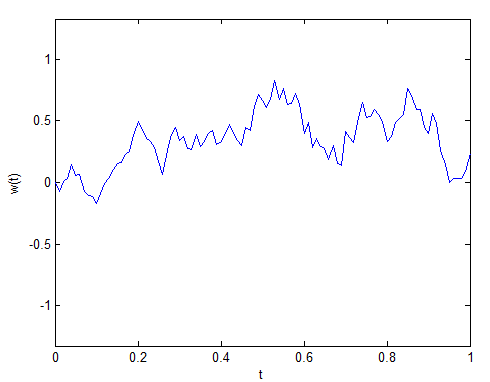
\includegraphics[width=\linewidth]{brownian.png}
\caption{Brownian motion with N=100}
\endminipage\hfill
\minipage{0.5\textwidth}
  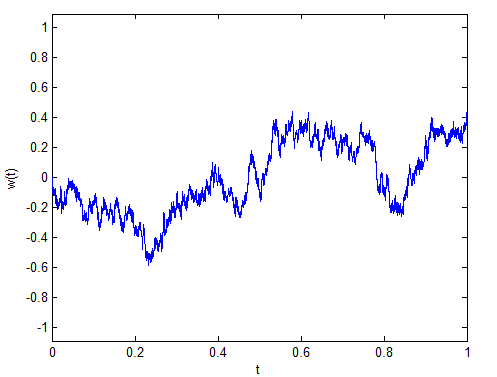
\includegraphics[width=\linewidth]{brownianN.png}
  \caption{Brownian motion with $N=10^4$}
\endminipage\hfill
\end{figure}

The simulation of a Brownian motion is totally described by equation  \eqref{broawnian}. We define time as a number of discrete interval of lenghth $\Delta t$ and in each time the general increment $\Delta W_t$ is given by multiplying  a standard normal random variable by $\Delta t$. We can remark that as N becomes larger, the length of each interval becomes arbitrary small and the process become more continuous. \\


To derive the Black-Scholes formula, some assumptions on the assets and the market have been made (these assumptions are detailed in Hull's book chapter: 12, 13, 14):
\begin{itemize}
\item Returns are log-normally distributed.
\item The options are European and can only be exercised at the expiration date(the last date on which the holder of the option may exercise it according to its terms).
\item The stock pays no dividend during the life of the option.
\item The volatility is constant for any strike and maturity.
\item The short-term interest rate (the risk-free rate r) is known and constant through time.
\end{itemize} 


It can be shown that under these assumptions and under the risk neutral valuation theorem\jcom{cite! Also explain why you need a risk neutral valuation theorem to solve a stochastic differential equation} the solution of the stochastic differential equation (1.1) is :
\begin{gather}
S_t= S_0 e^{(\mu-\frac{\sigma^2}{2})t+\sigma W^{\mathbb{P}}_t}
\end{gather}
where $W_t^{\mathbb{P}}$ is a standard Brownian motion under the risk neutral measure $\mathbb{P}$ \jcom{What does it mean when you say that something is a standar Brownian motion under some measure? How is this different from the statement you amde about Brownian motion earlier?} defined on the following probability space ($\Omega, \mathbb{P},\mathfrak{F}$),$\mathbb{P}$ is a probability distribution determined according to the hypothesis of absence of arbitrage and $\mathfrak{F}$ is a filtration that contains the information available at time t\\
For the Black and Scholes model, it holds that : 
\begin{gather}
X_t=log(\frac{S_t}{S_0})=(\mu-\frac{\sigma^2}{2})t+\sigma W^{\mathbb{P}}_t
\end{gather}

Let us denote the price of a European call for any $ t \in [0, T]$ by $C(St, K,T)$, then $C(St, K,T)$ is defined as the discounted expected value of $(S_T-K)^+$ under the risk-neutral probability measure $\mathbb{P}$,\\
\begin{align}
\text{C}(St, K,T)=& e^{-r \tau} \text{E}^P[(S_t-K)^+|\mathfrak{Ft}] \nonumber \\ 
&=e^{-r \tau} \text{E}^P[(e^X_t-K)^+|\mathfrak{Ft}] 
\end{align}


Developing this conditional expectation and using the Girsanov theorem (Wang,2014) to define an equivalent risk neutral measure $\mathbb{Q}$ will lead to the following price:
\begin{gather}
\text{C}(St,K,T)= S_0 \text{N}(d_1) - K e^{-r \tau} \text{N}(d_2)
\label{call}
\end{gather}

where $ d_1= \frac{ln\frac{S_0}{K}+r+\frac{\sigma^2}{2}T}{2} $ and $d_2 = d_1-\sigma \sqrt{T} $ \\
$ S_0$ is the current stock price, T is the time to maturity, $\sigma$ is the stock price volatility,$N(x)$ is the cumulative probability distribution function for the standard normal distribution. The price of the European put option can
be computed by the Put-Call parity.The 
\begin{gather}
P(St,K,T)= -S_0 \text{N}(-d_1) + K e^{-r \tau} \text{N}(-d_2)
\label{put}
\end{gather}
We can remark that the expected return $\mu$ does not appear in the Black-Scholes equation. This means the pricing formula is independent of the individual’s preference. 
\textcolor{blue}{we use the Girsanov theorem in the calculation of the right side of the expectation in the price formula, 
Where did the dependence on expected returns vanish? }
\jcom{Please state the Girsanov and Risk neutral valuation  theorems and justify them. One way of doing so would be to show that
their assumptions hold for the case in question.}

\section{The Essence  of the Black-Scholes-Merton Model}
\begin{itemize}

\item The Black-Scholes equation applies to a large variety of derivative assets. What distinguishes the different assets are the boundary conditions.
\item The formula \eqref{call} and \eqref{put} can be easily modified when the interest rate is stochastic or a function of t, when the stock gives dividend or when the option is American.

\item  In the Black-Scholes model, the market operates continuously with the share price following a continuous Ito’s process.  This suggests that continuous trading promotes price efficiency and helps investors to set their preferences.
\end{itemize}

These properties together with its simplicity make the Black-Scholes pricing formula very popular among practitioners for pricing options. 
\section{ Limitations of the Black Scholes Merton Model }
\begin{itemize}
\item \textbf{Non constant volatility}:
Although the Black-Scholes formula is powerful to price stock options, it is widely believed and experimentally verified  that stocks do not have a constant spot volatility, rather this parameter varies with time, e.g. Hull and White(1987), Danilo and Spokoinyi (2004),Goldentyer, Klebaner and Liptser (2005).This may systematically misprice the options and cause the biases of the Black-Scholes model. 


\item \textbf{Non complete market}:
The Black-Scholes-Merton  model assumes that the market is complete,i.e.  that any contingent claim can be perfectly hedged, but if we consider the real situation , the stock price can increase or decrease
lightly like it can fall relatively quickly.So,it is not possible to be hedged against all of these states
simultaneously. The impossibility of perfect hedging means that the market is incomplete Hence, it makes much more sense to use incomplete market models where the risk of hedging can be quantified rather than sticking to complete market models where the risk of hedging is by definition zero,more general Levy models  are examples of incomplete models. 


\item \textbf{Non Log-normal Distributed returns}: If the stock price follows a geometric Brownian motion with drift  as in equation $(1.1)$, the stock price is log-normally distributed, or, the logarithmic return is normally
distributed.Generally,when dealing with an asset price,this is a poor approximation because, returns often have an excess kurtosis and a non zero skewness values.

\item \textbf{Non continuous process}:
In traditional Brownian diffusion model, price movements are allowed with  small magnitude in short period of time. But in real markets, prices may be have big jumps ,a sudden dramatic decline in short time periods.A good model must be allow for discontinuities and jumps in price process.

\end{itemize}

\chapter{Lévy processes and financial modeling}

Generally, is always be more reliable to model prices with a stochastic process involving jumps in order to describe  market fluctuations.
Lévy processes, are in fact a valuable tool in financial modeling, because they  provide us with an appropriate
framework that describes adequately real time series.\\


This section defines Lévy processes , discusses some of their fundamental properties and introduces some examples like Compound Poisson processes in order to study the use of Lévy models in two categories of financial modeling with jumps :Jump diffusion and Infinite activity Lévy processes.

\section{ Lévy processes }

A Lévy process is a continuous time stochastic process defined on filtered probability spaces$(\Omega,\mathfrak{I},\mathfrak{I}_{t>0},P)$ ,it has the following properties:\\

i)$t \rightarrow X _t$ has cadlag paths, i.e. right-continuous with left limits.\\
ii) $X_0=0$.\\
iii) $X$ has an independent increments, i.e.$ X_t- X_s$ independent from \{ $X_u,{ u \leqslant s}.$\}\\
iv) X has stationary increments $X_t-X_s$ has the same distribution as $ X_{t-s}.$\\
v) X is stochastically continuous,lim $\lim\limits_{k \rightarrow +\infty}$ $P(|X_{t+k}-X_t|  \geqslant \epsilon)=   0 $   $   \forall       \epsilon > 0.$

The fourth property does not imply that the sample paths of $ X_t$ are continuous , it can be regarded as a way to exclude jumps at known time. It means that, at a given time $t$, the probability of seeing a jump is zero, discontinuities occur just at random times.\\

\section{Properties of  Lévy processes :}
\jcom{How exactly are the following properties different in kind from the ones already given?}
$\bullet$ \jcor{Let's}{Let} $(X_t)_{t \geqslant 0}$ be a Lévy \jcor{pocess}{process} on $\mathbb{R}^d$. The every Lévy process can be represented in the following form :
\begin{gather}
X_t= \mu t+ \sigma W_t + \int_0^t \int_{\mathbb{R}/\{0\}} (x-h(x))\nu(x) dx ds 
\end{gather}
where $ W_t $ is continuous geometric \jcom{why geometric?} Brownian motion that can be characterized by two parameters: the drift $\mu$ and the volatility $\sigma$, $\nu(x)$ is a measure on $\mathbb{R}$ called the Lévy measure and  $\int_0^t\int_{\mathbb{R}/\{0\}}(x-h(x))\nu(x) dx ds$ represents the jump part in the process $X_t$. h(x) in an arbitrary truncation function introduced to ensures that the integral part in the Lévy process is integrable.\\
\jcom{}{what is $h$?}


$\bullet$ To count the number of jumps, a Lévy measure is defined via the above formulation :

\begin{gather}
\nu(A)=E[\#\{t \in [0 1]: \Delta X_t \neq 0 , \Delta X_t \in A]
\end{gather}
\jcom{}{Why such definition? Would this not imply an infinite activity for a jumpless model?}
$\nu(A)$ represents the expected number, per unit time, of jumps whose size belongs to $A$.\\
$\bullet$ The distribution of a Lévy process is characterized by its characteristic function, the latter is defined such that :\\
\begin{gather}
\Phi_t(z)=\Phi_{X_t}(z)=E[ e^{izX_t}]
\end{gather}
$\bullet$ There exists a continuous function $\psi $  :$\mathbb{R}^d  \rightarrow \mathbb{R} $, called the characteristic exponent of $X_t$ ,such that:\\
\begin{gather}
E[ e^{izX_t}]= e^ {t \psi (z)}
\end{gather}
\jcom{}{Under which regularity assumptions does this hold true?}\\
\textbf{ Lévy-Khintchine representation} :\\

$\bullet$ If  $X = (X_t)_{t\geq 0}$  is a Lévy process, then its characteristic function  $\nu_{X_t}(z)$ \jcom{}{This is now the third
notation for a characteristic function, is there a subtlety that I am missing?}  is given by

\begin{equation}
\Phi_t(z)=\mathbb{E}\Big[e^{iz X_t} \Big] =e^ {t \psi (z)}
\end{equation}
\begin{equation}
\psi (z)= \mu iz - \frac{1}{2}\sigma^2  z^2 + 
\int_{\mathbb{R}\backslash\{0\}} \big( e^{izx}-1 -iz h(x)\big)\,\nu(dx) 
\end{equation}

This Lévy–Khintchine representation is fully determined by the Lévy–Khintchine triplet $(\sigma^2,\nu, \mu)$ where $\mu \in $ $\mathbb{R}$ is called the drift term, $\sigma$ the Gaussian or diffusion
coefficient and $\nu$ is the Lévy measure. This triplet is unique for every Lévy process $(X_t)_{t\geq 0}$.\\
$\bullet$ The Lévy measure has no mass at the origin and satisfies the following integrability condition :
\begin{multicols}{2}\noindent
\begin{equation}
 \nu( \{0 \}) = 0
\end{equation}
\begin{equation}
\int_{\mathbb{R}\backslash\{0\}} \big( min \{x^2,1\} ,\nu(dx) < \infty  \Big)
\end{equation}
\end{multicols}

$\bullet$ According to the Lévy Khintchine representation
\jcom{cite!}
, the characteristic exponent of every Lévy process can be written as the sum of the characteristic exponent of a Brownian motion with drift and the characteristic exponent of a jump component.
$$\psi_B (z)= \mu iz - \frac{1}{2}\sigma^2  z^2 $$
$$\psi_{jump}(z)=\int_{\mathbb{R}\backslash\{0\}} \big( e^{izx}-1 -iz h(x)\big)\,\nu(dx)$$
\jcom{}{Use mathrm for the english subscripts in formulas}

\textbf{Finite/Infinite activity and variation }\\

Considering,$X_t$, a Lévy process with a characteristic triplet $(\sigma^2,\nu, \mu)$ .As we have seen before, the Lévy measure represents the expected number of
jumps of a certain magnitude in a time interval of length 1. Thus, we are able to disguish the class of the Lévy process by reading the lévy measure:
\begin{enumerate}

\item If $\nu$ is a finite
measure,  $\nu(\mathbb{R})= \int_{\mathbb{R}} \nu(dx) < \infty$, then $X_t$ has a finite number of jumps on every finite interval, it is called \emph{finite activity Lévy process}.In this case we dot not need a truncation function $h(x)=0 $.

\item If $\nu$ is an infinite
measure, $\nu(\mathbb{R})=\infty $, an infinite number of jumps have occurred , $X_t$ is then called $\emph{infinite activity Lévy process}$. In this case, conditions $(2.7)$ and $(2.8)$ are no more sufficient to ensure the convergence of the integral part in the Lévy process, some conditions will be imposed on the measure $\nu$ under which we keep the same decomposition of $X_t$ as in $(2.1)$. 

\item if $\sigma = 0$ and $\int_{\mid x\mid
\leqslant1} x\nu(dx) < \infty $, then the path of $X_t$ a has finite variation.
\item if $\sigma \neq 0$ or $\int_{\mid
x\mid
\leqslant
1} x\nu(dx) = \infty $, then the
path of $X_t$ has an infinite variation.
\end{enumerate}
\chapter{ Financial Modeling with Lévy Processes }

After discussing general properties of Lévy processes, we can now give some tractable examples of Lévy processes that can be used in basic financial models and emphasize the different relations between them\jcor{}{.}\\
All the models that will be discussed belong to a family of Lévy processes called “exponential Lévy processes”, under which the dynamic of the underlying stock prices are given by: 
\begin{equation}
S_t= S_0e^{X_t}
\end{equation}
where $X_t$ is a Lévy process under the risk-neutral measure  $\mathbb{Q}$ with
characteristic triplet $(\sigma^2,\nu, \mu)$.
\jcom{}{Isn't the risk-neutral dynamic independent of the expected return?} The log returns log($S_{t}/S_0$) of such a model
follow the same distribution of the Lévy process $X_t$.
\section{Examples of Lévy process }
\subsection{Poisson process}
The Poisson process counts the number of arrivals in particular time interval.\\
To describe it more clearly, we consider a continuous time arrival process: $ W(u)=\delta(u)$. It is simply an impulse function
\jcom{}{Impulse function is not really a function} every time an event occurs:
\begin{figure}[H]
\centering
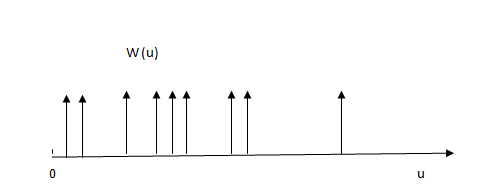
\includegraphics[scale=0.7]{arrival.png} 
\caption{An arrival process in the interval time [0 u]}
\end{figure}

The Poisson process $X_t$ will be the integral of this continuous time arrival process between 0 and t :\\
$X_t=\displaystyle \int_{0}^{t} W(u) \, \mathrm{d}u=\displaystyle \int_{0}^{t} \delta(u) \, \mathrm{d}u$ , which represents the total number of arrivals up to  time t.\\


\begin{figure}[h]

\centering
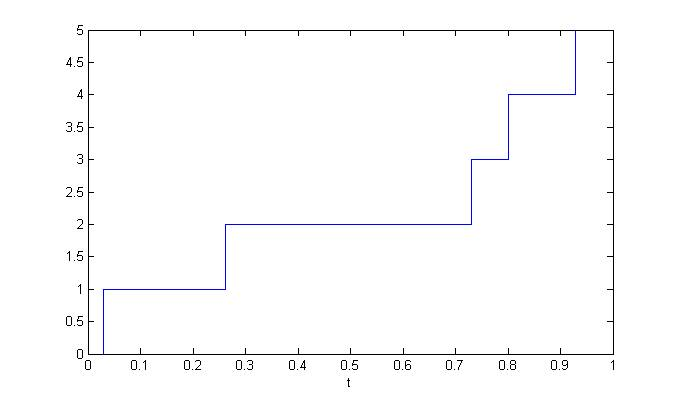
\includegraphics[scale=0.7]{poisson.jpg} 
\caption{Path of Poisson process with intensity $\lambda = 8$}
\end{figure}

As we can see, $X_t$ is continuous time discrete valued process with independent jumps of size one. $X_t$ can be characterized by :\\

i) The waiting time between two successive jumps, it is a random variable called the interarrival time. \\
ii) The interarrival time in the Poisson process follows an exponential distribution that has a very important characteristic called "memorylessness" 

\begin{gather}
 \forall t > s > 0, \text{P}(T > t + s|T > t) = \text{P}(T > s)
\end{gather}

iii) Every Poisson is characterized by a rate parameter $\lambda$, also known as the intensity of the process such that the number of arrivals in time interval $[t, t + \epsilon]$ follows a Poisson distribution with associated parameter $\lambda \epsilon$ . This relation is given as
\begin{gather}
 P [N(t+ \epsilon) - N(t) = k] = \frac{e^{-\lambda \epsilon} (\lambda \epsilon)^k}{k!}  \qquad k= 0,1,\ldots,
\label{foo}
\end{gather} 
 \jcom{For infinitesimal intervals, $k \geq 2$ is negligible!}
 
\subsection{Compound poisson process}
Let $X_t$ be a Compound Poisson process with intensity $\lambda$ and jump size distribution F, then $X_t$ will be defined as the sum of N(t) jumps arriving randomly according to a Poisson process and having random size specified with the probability distribution F.
\begin{gather}
X(t) = \sum_{i=1}^{N(t)} Y_i
\end{gather}
where,  $\{\,N(t) : t \geq 0\,\}$ is a Poisson process with rate $\lambda$, and $ \{\,Y_i : i \geq 1\,\}$ are independent and identically distributed random variables, with distribution function F.\\
In other words, we could say that a Compound Poisson process is a Poisson process except that the jumps have a random size.

\begin{figure}[h]

\centering
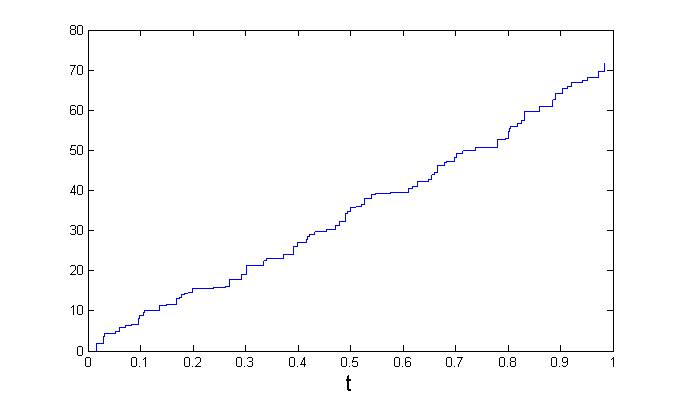
\includegraphics[scale=0.7]{compoisson.jpg} 
\caption{Compound Poisson process with intensity $\lambda=8$
\jcom{How likely is it to have approximately ten times as many jumps as the mean, such as in the picture? Please elaborate on the scheme of simulation you use to produce these plots?}}
\end{figure}
\jcom{What is the distribution of these jumps? Also: how likely is it according to \ref{foo} to have this many jumps? Avoid
pixel rasterisations, when possible. Also, avoid pixel rasterisations like this, there are multiple schemes like tikz and pgfplots that you 
can use to avoid the pixelation of an image.}

\section{Lévy processes in Finance}

Two categories of Lévy processes are used to describe the evolution of market prices. 
The first category is called "Jump-diffusion models": these models have rare jumps and random evolution between the jump times. 
\jcom{Why is infinite jump activity diffusive model not possible?}
Such a model can be modeled by a Brownian motion with drift plus a jump part, which is a compound Poisson process .\\

Contrary to Jump-diffusion models, the second category of Lévy processes consists of models with infinite number of jumps in every time interval,
\jcom{almost surely} called "Infinite activity models".Some of these models could be modeled without Brownian component. Hence, the jump part is the deterministic of the price dynamic, this subcategory is called "infinite activity pure jump models". \jcom{What does it mean that the jump part is the deterministic of something?}
\subsection{Jump diffusion models}
As their name would suggest, these models contain  a diffusion part represented by a Gaussian process (Brownian motion) accentuated by a finite number of jumps(Compound poisson process) with size distribution F.      \\


A Lévy process of jump-diffusion type has the following form: 
\begin{gather}
X_t = \mu t+\sigma W_t+\sum_{i=1}^{N(t)} Y_i
\label{bar}
\end{gather}

where $\mu \in \mathbb{R}, \sigma \in \mathbb{R_+}$, $W_t$ is a standard Brownian motion, $N =(N_t)_{t \geqslant 0}$ is a Poisson process with parameter $\lambda$ (i.e. $E[N_t] = \lambda t$) and $Y = (Y_t)_{t\geqslant 1}$ is an i.i.d. sequence of random variables with probability distribution F. All sources of
randomness $(W_t,N_t,Y_t)$ are mutually independent.

Two famous models of Lévy processes of jump diffusion type are used in modelling the log-price dynamic : The Merton jump-diffusion model and the Kou model.\\

\large\textbf{Merton model}\\


Merton was the first to use a discontinuous price process to model asset returns. (Merton 1976) assumed that the total change in the stock price is posited to be the composition of two types of changes:\jcom{itemize?}(1)The ‘normal’ vibrations in price, for example, due to a temporary imbalance between supply and demand, changes in capitalization rates, changes in the economic outlook, or other new information that causes
marginal changes in the stock’s value. In essence, the impact of such information is to produce a marginal change in the price
(almost certainly). This component is modeled by a standard geometric Brownian
motion with a constant variance per unit time and it has a continuous sample
path. (2) The ‘abnormal’ vibrations in price are due to the arrival of important new information about the stock that has more than a marginal effect on price. By its very nature, important information arrives only
at discrete points in time. This component is modeled by a ‘jump’ process reflecting the non-marginal impact of the information.\\


According to the Merton model, the decomposition of the process in given by :
\begin{gather}
X_t = \mu t+\sigma W_t+\sum_{i=1}^{N(t)} Y_i
\label{baz}
\end{gather}
\jcom{How are \ref{bar} and \ref{baz} different?}
where the jump \jcor{size}{sizes} are assumed to have a Gaussian distribution F :
\begin{gather}
F(x) = \frac{1}{\sqrt{2\pi\sigma^2} } e^{ -\frac{(x-\alpha)^2}{2\sigma^2} }
\end{gather}
\jcom{Why constrain to the case in which the jump sizes variance equals the variance of the wiener process?}
Thus, $Y_i  \sim N(\alpha,\sigma^2)$ and the Lévy density :
\begin{gather}
 \nu(x)=\lambda F(x)=\lambda\frac{1}{\sqrt{2\pi\sigma^2} } e^{ -\frac{(x-\alpha)^2}{2\sigma^2} }
\end{gather}
This allows to obtain the probability density of $X_t$ as an expansion series: 
\begin{gather}
p_t(x)=e{-\lambda t} \sum_{k=1}^{\infty} \frac{(\lambda t)^k  e^{ -\frac{(x-\mu t-\alpha k)^2}{2\sigma^2+k \delta^2}}}{k!  \sqrt{2\pi(\sigma^2+k \delta^2)}}
\end{gather}

Taking the parameter values of $S\&P500$ Market from (Andersen and Andreseasen 2001):
\jcom{please include the proper reference}

$ r =5.59 \%,\quad \sigma=17.65\%,\quad  \lambda=8.90\%, \alpha=-88.98\%,\quad  \delta=45.05\%  T=1 year $

we will obtain the following Merton processes. \\


\begin{figure}[h]

\centering
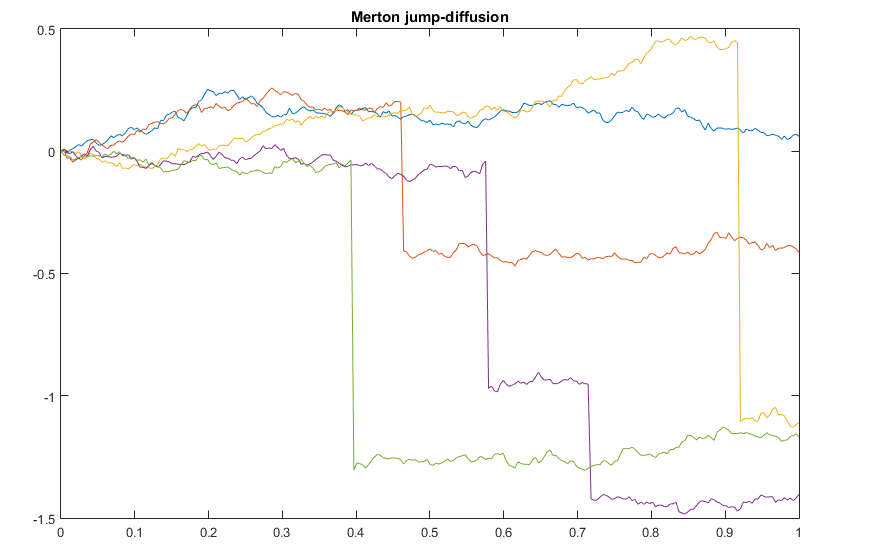
\includegraphics[scale=0.7]{merton.png} 
\caption{Simulated log-price sample paths with Merton model  $\lambda=8$}
\end{figure}
\jcom{Please explain how the simulated realisations have been obtained. Also, how likely is it that one obtains
five independent realisations of a Poisson process with expected number of jumps being 8, such that
all realisations have at most 2 jumps? I assume this probability to be negligible.}
In this graph, the log-price sample path is simulated 5 times in order to see to what extent the source of randomness can change and affect the log-price variation. 
\\


\large\textbf{Kou model}\\

Since the first discontinuous price process proposed by Merton, many researches have been conducted in order to generalize the Black-Scholes model and to incorporate more empirical features(skewness, excess kurtosis and stochastic volatility). This variety of alternative proposed models was presented in Hull (2000) \jcom{citation!}and just like the Black Scholes model they are usually designed to European call and put options.
Hence, it is impossible to derive an analytical solution using these models for other option type such that: American options, lookback options, and barrier options using \jcom{using what} .\\

It was in 2002 that S. G. Kou \jcom{citation!} proposed a jump-diffusion model for option pricing leading to an analytical solution for many option-pricing problems.

Kou demonstrated that double exponential jump size distribution performs well with different option classes  in \jcor{term}{terms} of accuracy and ease of implementation.

The Double Exponential Jump Diffusion Model is given by: 
\begin{gather}
X_t = \mu t+\sigma W_t+\sum_{i=1}^{N^*(t)} Y^*_i
\end{gather}
Where $W_t$ is \jcor{a}{} standard Brownian motion, $N^* =(N^*_t)_{t \geqslant 0}$ is a Poisson process with parameter $\lambda^*$ (i.e. $E[N_t] = \lambda^* t$) and the log jump sizes $\{Y^*_1 , Y^*_2 , ... \}$ are
independent identically distributed (i.i.d.) random variables such that $Y_i$ has a new double exponential distribution 
\begin{gather}
F(x)= p.\eta_1 \exp \left( -\eta_1 x \right) \mathbf{1}_{\{x\geqslant 0\}}+ q .\eta_2 \exp \left( -\eta_2 x \right) \mathbf{1}_{\{x < 0\}}
\end{gather}
$\lambda > 0,~ \eta_1 > 1, \eta_2 > 0$~,  
$(p,q) \geqslant 0,~ p+q=1$ are the probabilities of the upward and downward jumps of the stock price. So we can
express this also in this way:\\

         \[Y_i = \begin{cases} 
  \zeta^+ ~ with~ a~ probability ~ p \\
         \zeta^-  ~with ~ a ~ probability ~ q
         \end{cases}
          \]
$\zeta^+$ and $\zeta^+$, are exponentially distributed random variables with an expectation value of $\frac{1}{\eta_1}$ and $\frac{1}{\eta_2}$.\\

The lévy measure of the Kou model \jcor{will be defined as below}{is given as}:

\begin{gather}
 \nu(x)=\lambda F(x)=\lambda \big[ p.\eta_1 \exp \left( -\eta_1 x \right) \mathbf{1}_{\{x\geqslant 0\}}+ q .\eta_2 \exp \left( -\eta_2 x \right) \mathbf{1}_{\{x < 0\}}\big]
\end{gather}

Taking the values of Double Exponential Jump Diffusion Model  from (Kou 2002):\jcom{citation!}

$ \eta_1= 10,~\eta_2= 5,~\lambda=1,~\sigma= 16\%,~r=5\%,~ p=0.4,~ q=0.6 ~ and ~T=1 year $\jcom{why need for units for maturity} will lead to the following log-price process.

\begin{figure}[h]

\centering
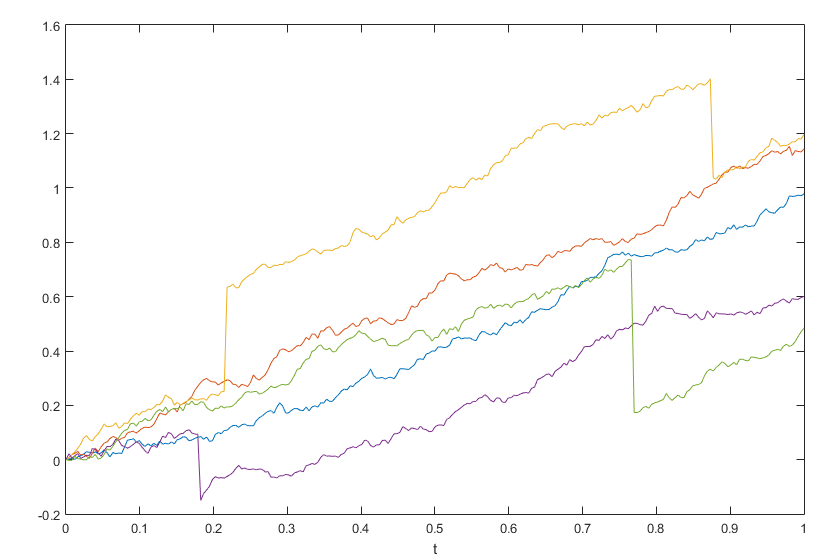
\includegraphics[scale=0.7]{kou.png} 
\caption{Simulated log-price sample paths with Kou model }
\end{figure}
\jcom{Once again, avoid pixel rasterisations. What are the parameters of this plot and how was it generated?}

The values of the parameters \jcor{was}{were} taken from these \jcom{which references?} references in order to be able to benchmark the forward results \jcom{which forward results?} with the exact option price calculated in these papers .

\chapter{Fourier Transform Methods For Option pricing }

Various methods can be used to price an option when the underlying
asset price process is modeled by a Lévy process. One can use the famous partial differential equations PDE  and solve it numerically with the finite differences methods which  can be difficult due to the presence of jumps (this approach can be used to solve derivative pricing problems that have, in general, the same level of complexity as those problems solved by tree approaches).~Another method is to use Monte Carlo simulation in order to simulate different paths of the risk neutral process and take the discounted value of the average to obtain the option price.~In spite of its efficiency, Monte Carlo simulation is known to be computationally intensive. \\

There are two reasons why one would choose Fourier transform approach for option pricing: while the first reason is overcoming the problem of unknown  probability density of some Lévy processes, the second reason looks more important, since the use of Levy-Khinchine formula allows us not only to recover the analytical expression of the characteristic function but also to take advantages from excellent numerical properties of the Fourier Transform approach: greater rate of convergence,use of the FFT algorithm, flexibility of moving from the real space to the Fourier space and and vice versa (the properties will be further detailed) . \\

This chapter will introduce Fourier transform approach and demonstrate its effective use for option pricing.~we will also explain the importance of Fast Fourier Transform algorithm FFT in calculating the anti-transform and reducing the overall complexity of the algorithm. We will detail all the numerical results for the Merton , the rest will be presented in the appendix part. 
\newpage
\section{Constructing risk neutral characteristic  function }

In order to use the Fourier approach for option pricing,  we will  evidently need an analytical expression of the characteristic function of the Lévy process for every model presented above.\\

Let's $X_t$ be a Lévy process under the risk neutral measure $\mathbb{Q}$(under which the discounted stock price is a martingale).~ $\mathbb{Q}$ can be obtained with  Girsanov theorem for Lévy processes (Jacod and Shiryaev,2003) or Esscher Transform approach ( Esscher, 1932).\\ 
We have mentioned in chapter(1) that the characteristic function of a $X_t$ takes the form of $e^{t \psi(z)}$
where  $\psi(z)$ is the characteristic exponent defined under $\mathbb{Q}$ by the Lévy Khintchine representation : 
\begin{equation}
\psi (z)= \mu iz - \frac{1}{2}\sigma^2  z^2 + 
\int_{\mathbb{R}\backslash\{0\}} \big( e^{izx}-1 -iz 1_{|x| \leq  1  } \big)\,\nu(dx) 
\end{equation}
We have also mentioned that we can divide $\psi (z)$ into two parts :
\begin{center}
$\psi(z)= \vartheta(z)+\phi(z)$
\end{center}
where $ \vartheta(z)$ is the drift part and $\phi(z)$ is the diffusion part 
\begin{center}
$ \vartheta(z)=t \mu iz$\\
$ \phi(z)= - \frac{1}{2}\sigma^2  z^2 + 
\int_{\mathbb{R}\backslash\{0\}} \big( e^{izx}-1 -iz 1_{|x| \leq  1  } \big)\,\nu(dx)$
\end{center}
It can be demonstrated that under the risk neutral martingale $\mathbb{Q}$
\begin{center}
 $\vartheta^{RN}(z)=i(r-\phi(-i))z=r-\frac{\sigma^2}{2}-\lambda \zeta=i\mu^{RN} z$ 
\end{center}
where $\zeta=\mathbb{E}(e^Y)-1$ and $\mu^{RN}$ is the corrected drift under $\mathbb{Q}~$~(risk neutral drift)and r is the risk free interest rate 

Thus we could conclude that under the risk neutral measure $\mathbb{Q}~$ the characteristic function can be redefined as :
\begin{equation}
\psi (z)= i\mu^{RN} z - \frac{1}{2}\sigma^2  z^2 + 
\int_{\mathbb{R}\backslash\{0\}} \big( e^{izx}-1 -iz 1_{|x| \leq  1  } \big)\,\nu(dx) 
\end{equation}

In the following table we define the risk-neutral characteristic functions for our three Lévy processes.
\begin {table}[h!]
\begin{center}
\renewcommand{\arraystretch}{2}
\begin{tabular}{|l|l|l|}
 \hline
   Lévy model  & risk-neutral drift & Risk neutral characteristic function   \\
 \hline
Merton model  & $r-\frac{\sigma^2}{2}-\lambda (e^{\alpha+\frac{\delta^2}{2}}-1)$ & $\psi (z)= i\mu^{RN}z - \frac{1}{2}\sigma^2  z^2 + \lambda (e^{i \alpha z - \frac{1}{2} \delta ^2 \sigma^2}-1)$  \\
 \hline
 Kou model  & $r-\frac{\sigma^2}{2}-\lambda \big(\frac{p \eta_+}{\eta_+ -1}-\frac{q \eta_-}{\eta_- + 1}-1\big)$ & $\psi (z)= i\mu^{RN}z - \frac{1}{2}\sigma^2  z^2 + i z \lambda \big(\frac{p}{\eta_+- i z}- \frac{q}{\eta_- + i z}\big) $   \\

\hline
\end{tabular}
\end{center}
\caption{Merton model , kou model and Gamma Variance model} 
\end{table}
\section{Option price}
Consider an asset whose price at time t is modeled under the risk neutral measure $\mathbb{P}$ by the stochastic process $S = (S_t)$
defined by $St = S_0 e^{X_t}$ , where $X = (X_t)$  is assumed to be a Lévy process whose
jump measure is $\nu$.\\

Assuming the risk-neutral dynamic for $S_t$, the price at time $t = T-\tau$  of a European option with payoff G and maturity time T is given by

\begin{gather}
\pi(\tau,x)= e^{-r\tau} \expp{G \parent{X_T}|X_{T-\tau} = x}
\label{price}
\end{gather}
where r is the short rate that we assume to be constant and $\tau$ : 0 <$\tau$ < T is the time to
maturity.

Consider $g$ as the reward function in log prices (ie, defined by $g(x) = G(S_0e^x)$). Now, take f to be defined as
\begin{center}
$f \parent{\tau,x} \equiv \expp{g \parent{X_T}|X_{T-\tau} = x}$
\end{center}

We can observe that f and $ \pi$ are related by :
\begin{gather}
\pi(\tau,S_0 e^x)= e^{-r\tau}f \parent{\tau,x}
\end{gather}
The value of the option $\pi$ is related to the risk-neutral density $p_T$ by:


\begin{align}
\begin{split}
\pi\parent{\tau,x} \equiv & e^{-r\tau}\expp{g \parent{X_T}|X_{T-\tau} = x}
\\
= &e^{-r\tau}\int_\R g\parent{y}  p_\tau \parent{y-x}  \d y
\\
=& e^{-r\tau}\int_\R (S_0 e^y-K)^+ p_\tau \parent{y-x}  \d y, ~~k=log (\frac{K}{S_0})\\
=& e^{-r\tau} \int_k^\infty (S_0 e^y-K) p_\tau \parent{y-x} \d y
\label{moneq}
\end{split}
\end{align}

(See Appendix \eqref{moneq} for details of the derivation of the discounted expected conditional terminal payoff).\\ 
It should be noted that the above price is homogeneous of order 1 with respect to the variable x . i.e.
$\pi(\tau, \lambda x) = \lambda \pi(\tau,  x) $
see (JOSHI) for the full demonstration. 
\section{Fourier Transform approach}

There are different conventions for the Fourier transform. In this section we consider the operator
$\cal{F}$ such that :

\begin{center}
$\cal{F}$$[f](w)= \int_\R e^{iwx}f(x) dx $
\end{center}
To recover the original function f, we define the inverse Fourier transform as

\begin{center}
$\cal{F}$$^{-1}[\hat{f}] (x) =\frac{1}{2\pi}\int_\R e^{-iwx}f(w) dw $
\end{center}


The principle of the Fourier Transform method is simple: instead of applying the direct discounted expectation, it is easier to compute the integral of its Fourier transform and after that we could recover the option price due to this characteristic:
\begin{center}
$\cal{F}$$^{-1}[\hat{f}] (x)=f(x)$
\end{center} 


From the previous derivation of the option price function eq ~\eqref{moneq}, we could remark that it is not square integrable. To obtain a square integrable function, we would consider a damped version of f defined by $f_{\alpha}(\tau,x) = e^{-\alpha x}f(\tau, x)$.We will discuss later  the choice of $\alpha$.

Now, having an integrable function $f_\alpha$ we can apply the operator $\cal{F}$, we will obtain :
\begin{gather}
\hat{f}_{\alpha}(w,\tau)=\int_\R e^{iwx} f_{\alpha}(x,\tau) dx 
\end{gather}


\begin{equation}
f_{\alpha}(x,\tau)=\frac{1}{2\pi}\int_\R e^{-iwx}\hat{f}_{\alpha}(w,\tau) dw
\end{equation}

Thus,\\
\begin{align}
f(x,\tau)= & e^{\alpha x} f_{\alpha}(x,\tau)\\
= & \frac{e^{\alpha x}}{2\pi}\int_\R e^{-iwx}\hat{f}_{\alpha}(w,\tau) dw
\label{souma}
\end{align}

We just have to derive an analytic expression of $f_\alpha(w,\tau)$ to put in the equation \eqref{souma} and get back the price of the option.

\begin{align}
\hat{f}_{\alpha}(w,\tau)= &\int_\R e^{iwx} f_{\alpha}(x,\tau) dx \nonumber
\\
= &  \int_\R \int_\R \expfs{- \damp x + i \omega x} g \parent{y}  p \parent{y-x} \d y \d \omega \nonumber
\\
= & \int_\R \int_\R \expfs{ i \omega x} g \parent{y} \expfs{-\damp y} \expfs{-\damp \parent{y
-x}}  p \parent{y-x} \d y \d \omega \nonumber
\\
= &\hat \ga \parent{\omega} \charFun{\tau}{\omega + i \damp} \nonumber
\\
= & \hat \ga \parent{\omega} \expfs{\tau \charExp{-i \parent{\omega+i \damp}} } \nonumber
\\
= & \hat \ga \parent{\omega} \expfs{\tau \charExp{\damp - i \omega} }.
\label{ghat}
\end{align}

Where $\charExp \omega $ is the characteristic exponent and $ \hat \ga \parent{\omega}$ is the Fourier transform of the damped terminal payoff (see Appendix \eqref{ghat} for further details). \\

Now we have an analytical expression of $\hat{f}_{\alpha}(w,\tau)$, to obtain the value function we have to employ the inverse Fourier transformation :

\begin{equation}
f_{\alpha}(x,\tau)=\frac{1}{2\pi}\int_\R e^{-iwx}\hat{f}_{\alpha}(w,\tau) dw
\end{equation}

or 

\begin{equation}
f_{\alpha}(x,\tau)=\frac{1}{\pi}\int_{0}^{\infty} Re[e^{-i \omega x}\hat{f}_{\alpha}(\omega,\tau)] ]dw
\label{DF}
\end{equation}

\section{The discrete Fourier Transform method DFT}

As it is not possible to compute the inverse Fourier transform analytically eq \eqref{DF}, we
approximate it by truncating and discretising the integration domain using the trapezoidal quadrature rule.\\ 

In fact, the trapezoidal rule is a technique for approximating an integral by interpolating between N  points using a straight line that relates each two successive points. 

The trapezoidal rule can be written in the following form :\\
  
Let $I$ be a definite integral:
\begin{center}
$I=\int_{a}^{b} f(x) dx$
\end{center}  
I is approximated by 
\begin{center}
$I ~\approx ~ \sum \limits_{k=0}^{N-1} h_k f(x_k)$
\end{center}

where $\omega_k$ are the weights of $f(x_k).$ 


Generally, we choose $x_k$ as equidistant points $x_k= \big ( a+k \frac{b-a}{N}\big ) _{0 \le k \le N-1}$ having the same weight $h=\frac{b-a}{N}$\\
Then ,
\begin{gather}
I ~\approx ~ h \sum \limits_{k=0}^{N-1} f(x_k)
\label{approx}
\end{gather}

For our case,we will apply another version of the trapezoidal rule , the midordinate integration rule. Instead of evaluation $f$ at $x_k$ we will evaluate it at the midpoint defined by :
 $ x_k= \big ( a+(k+\frac{1}{2}) \frac{b-a}{N}\big ) _{0 \le k \le N-1}$.\\
 
Applying (\ref{approx} ), gives the the following approximation :
\begin{align}
f_{\alpha,\Delta \omega, N}=&\frac{\Delta \omega}{2\pi} \sum \limits_{k=-N}^{N-1} e^{-i(k+\frac{1}{2}) \Delta \omega x }\hat{f}_{\alpha}(\omega,\tau)
\\
=& \frac{\Delta \omega}{\pi} \sum \limits_{i=0}^{N-1} \text{Re}[e^{-i(k+\frac{1}{2}) \Delta \omega x }\hat{f}_{\alpha}((k+\frac{1}{2}\Delta\omega ),\tau)]
\label{fret}
\end{align} 
Thus the option price is: 
\begin{center}

$f_{\Delta \omega, n}(x,\tau)= e^{\alpha x}f_{\alpha,\Delta \omega, n}(x,\tau)$
\end{center}
 
 Here we can see that [a,b]=[$\omega_{min},\omega_{max}$]
 where,
\begin{center}
 $\omega_{min}=(-N+\frac{1}{2})\Delta \omega$\\
 $\omega_{max}=(N-\frac{1}{2})\Delta \omega$
\end{center}


The efficiency of DFT lies in the choice of an appropriate truncated interval and the number of quadrature points. But before deciding on the truncated interval we need to identify the shape of the symmetric function inside the sum $ \text{Re}[e^{-i(k+\frac{1}{2}) \Delta \omega x }\hat{f}_{\alpha}((k+\frac{1}{2}\Delta\omega ),\tau)$ , it will denoted by $H(\omega)$\\


Riemann-Lebesgue Lemma (Stenger, 1993) states that :\\ If f $\in L^1(\mathbb{R}$) and F is the Fourier transform of f, then  $\lim\limits_{x \rightarrow \pm \infty} F(\omega)=0$\\

Thus we could say that $H(\omega)$ is vanishing at infinity and starting from a certain point we can truncate it. In order to better choose [$\omega_{min},\omega_{max}$] , we represent below H($\omega$) for the Merton model. The function is plotted for the same previously chosen values of the Merton model parameters taken from (Andersen and Andreseasen ,2001):\\ 
$ r =5.59 \%,\quad \sigma=17.65\%,\quad  \lambda=8.90\%, \alpha=2,\quad \upsilon = -88.98\%,\quad  \delta=45.05\% \quad T=1 year,\quad x=log(\frac{S_t}{S0})=1 $ 
\\
\begin{figure}[H]
\centering
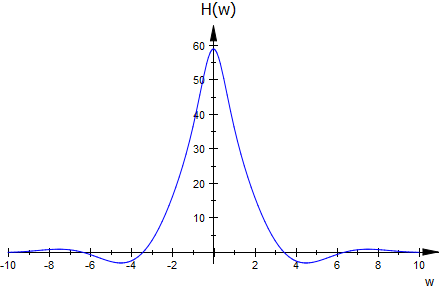
\includegraphics{H.png} 
\caption{Shape of H($\omega$)}
\label{H(w)}
\end{figure}

 
From the graph we can say that beyond $\omega=\omega^* $, H becomes of negligible values, thus we can set
\begin{center}
$\omega_{max}=(N-\frac{1}{2})\Delta \omega=\omega^*$\\
$\Delta \omega= \frac{\omega_{max}}{N-\frac{1}{2}}$
\end{center} 

Once $\omega^*$ is picked up we just need to choose the number of quadrature points N and we will obtain an approximated option price .
\section{Closed-Form option valuation for the Merton Model}
In order to evaluate the efficiency of the DFT method we need to  compare its results with a reliable reference value, this value will be also used for the subsequently presented methods.\\
Merton assumed in his jump diffusion model that jumps are Gaussian.~Based on this assumption, he developed a closed-form solution for an option as a series expansion of weighted Black and  Scholes prices. The closed form formula is explained below and the whole derivation is in (Merton,1975).
\begin{align}
\label{sum2}
\pi(S,\tau)=& e^{-r\tau} \sum \limits_{n=0}^{\infty} P(n~jumps~occurs)~\mathbb{E}(max(S-K,0)|k~jumps) \nonumber \\
=& e^{-r\tau} \sum \limits_{n=0}^{\infty} \frac{e^{-k \lambda \tau}(\epsilon \lambda \tau)^n}{n!} ~ \mathbb{E}_0(max(S-K),0|n~jumps)\nonumber \\
=& e^{-r\tau} \sum \limits_{n=0}^{\infty} \frac{e^{-k \lambda \tau}(\epsilon \lambda \tau)^n}{n!} BS(S,\tau,K,\sigma_k,r_k)
\end{align}

Where,
\begin{center}
$k=E^Y$\\
$\sigma_k^2=\sigma^2+\frac{k}{\tau} \delta^2$\\
$r_k=r-\lambda(E^Y-1)+k \frac{log(\epsilon)}{\tau}$\\
\end{center} 
$E^Y$ is the mean of the jump size, for the Merton model $E^Y = e^{\upsilon+\frac{1}{2}\delta^2}$(the jump $\sim$ N($\upsilon,\delta^2$) )

Although an infinite series appears in the formula of $\pi$, the following graphs proves that  generally within  10 to 15 iterations the price converges to a certain value that will be later considered  as a reference for the other methods.
N denotes the number of iterations that are carried out in the sum \eqref{sum2}.



Using Andersen $\&$ Andreseasen parameters, we will get the following figure: 

\begin{figure}[H]
\centering
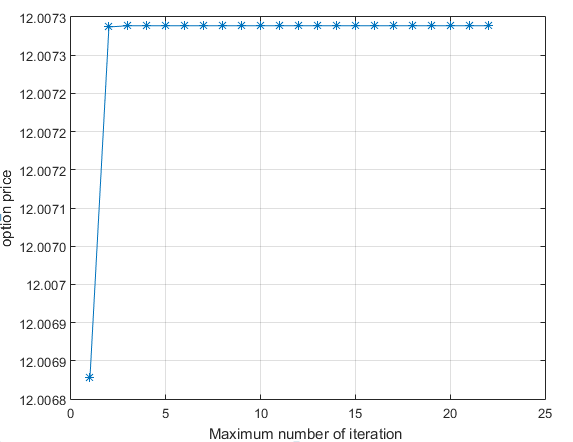
\includegraphics{maxiteration.png} 
\caption{ European option price with the Merton extension series}
\end{figure}


\section{Evaluation of the DFT methods }
\textbf{Error Analysis }
To evaluate the DFT we need to identify and quantify the total erro $\epsilon$ of the method.
 $\epsilon$ can be split into a sum of two terms: the quadrature and truncation errors denoted respectively by $\epsilon_Q$ and $\epsilon_T$. The former is the error from the approximation of the integral in \eqref{ghat} by an infnite sum, while the latter is due to the truncation of the infnite sum to a sum over N points .\\
\begin{center}
$|\epsilon|=|\epsilon_Q+\epsilon_T|$\\
$|\epsilon| \leq |\epsilon_Q|+|\epsilon_T|$\\
$\epsilon_Q=e^{\alpha x }|f_{\alpha}(\tau,x)-f_{\alpha,\Delta w }(\tau,x)|$\\
$\epsilon_T=e^{\alpha x }|f_{\alpha,\Delta w }(\tau,x)-f_{\alpha,\Delta w, N }(\tau,x)|$
\end{center}


Trefethen and Weidman proved that Trapezoidal rule converges exponentially when applied to analytic functions.
Before detailing more we need to define the following notion, denote by $A_a$, with a > 0, the strip of width 2a around the real line:
\begin{center}
$A_a \equiv \{z \in \mathbb{C}: Im [z] < a\}$
\end{center}
The following theorem presents conditions under which the quadrature error goes to zero
at a spectral rate as $\Delta \omega$ goes to zero. Three hypothesis must be admitted in order to use this error bound estimation :
 \begin{itemize}
\item The characteristic function of the random variable X has an analytic extension
to the set.
\item The Fourier transform of g(x) is analytic in the strip $A_a$ and
\item $\lim\limits_{\omega \rightarrow +\infty} sup _{\beta \in (-a,a)} |\hat{f}_{\alpha}(\tau, \omega+i\beta)|=0$
\end{itemize}

Then consider $M_{\alpha, a}(\tau,x)=sup _{\beta \in (-a,a)} \int_\mathbb{R} | e^{-i(\omega+i\beta x)}\hat{f}_{\alpha}(\tau, \omega+i\beta) |\,
 \mathrm{d} w$.

Then, for any $\Delta \omega$ > 0, $f_{\alpha,\Delta w }(\tau,x)$ as defined by \eqref{fret} exists and satisfies
\begin{gather}
|f_{\alpha}(\tau,x)-f_{\alpha,\Delta \omega }(\tau,x)| < e^{\alpha x} \frac{M_{\alpha, a}(\tau,x)}{\pi(e^{\frac{2\pi a}{\delta \omega}}-1)}
\end{gather}
Returning back to our function H(w),we know that it is analytic in the strip $A_a$, and concerning the last hypothesis, the graph \eqref{H(w)} proves the vanishing property of H. Thus we can substitute the bound provided by Trefethen and Weidman theorem for our quadrature error .
For what concerns the truncation error we can say that H(w) decays rapidly. we could then truncate the infinite series at quite small |k| with negligible effect.


\begin{figure}[H]

\centering
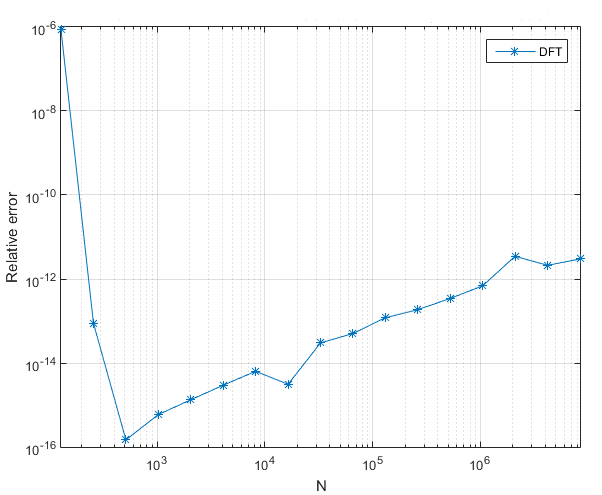
\includegraphics{DFT.png} 
\caption{Error the DFT method}
\end{figure}





\section{Fast Fourier Transform Algorithm}
The Fast Fourier Transform algorithm is numerically, efficient method to calculate Discrete Fourier Transform DFT. It was originally developed by Gauss (1805), but not recognized until Cooley and Tukey worked on it(1965).

The DFT is known to approximate a continuous Fourier transform (CFT) to its discrete counterpart:

\begin{equation}
\int_{0}^{\infty} e^{-iwx}f(x) dx ~\approx ~ \sum \limits_{k=0}^{N-1} e^{-i \frac{2\pi}{N}kj} f(x_k)~~~ k=0,...,N-1
\label{FFT}
\end{equation}


If we consider how much complication is involved in this DFT we will find :

- N complex multiplications.\\
- N-1 complex additions. \\
- We need to repeat that for k=0,...,N-1\\

In total, we need ~$O(N(N+N-1)) = O(N^2)$  operations to evaluate the quadrature rule for N asset value points. The FFT reduces significantly the complexity from order $O(N^2)$ to order $O(N log_2N)$.\\
 Although it appears to  have the same computation time, will figure out that FFT makes  a big difference when N is very large.
\begin {table}[h!]
\begin{center}
 \begin{tabular}{|c |c |c |} 
 \hline
N & $N^2$ & N $log_2 N$ \\ [0.5ex] 
 \hline
 100 & $10^6$ & $10^4$ \\ 
 \hline
 $10^6$ & $10^{12}$ & $20.10^6$ \\
 \hline
 $10^9$ & $10^{18}$ & $20.10^9$  \\
 \hline
\end{tabular}
\end{center}
\caption {DFT Vs FFT computation time }
\end{table}


 As we see when N is large the FFT reduces the amount of time that usual DFT takes to perform the option price. we will also see that it provides an efficient way of computing the previous bound eq \eqref{FFT} for several values of x at the same time.\\

 We can clearly notice that the summation in \eqref{fret} is not a direct application of the FFT algorithm. We need to modify it in a way to enter a vector and a matrix as inputs in order to obtain a sequence of option prices for different spot values of the asset. 

We consider the following frequency and log-price domains :
\begin{center}
$\omega_k=\omega_{min}+k\Delta \omega$ for ~~~ k=0,...,~N-1\\
$x_j=x_{min}+j\Delta x$ ~~~ j=0,...,~N-1
\end{center}


Here $\Delta x$ and $\Delta \omega$ are the grid spacing or the discretization steps,    $\omega_{k_{0\leq k <N }}$ and $x_{j_{0\leq j <N }}$ are equidistant points, $\omega_{min}$ and $x_{min}$ are the lower limits of the integration domains.\\

Using these grids, we can rewrite the integral that appears in the formula \eqref{fret} as follows:

\begin{align}
f_{\alpha,\Delta \omega, n}(x_j)=&\frac{\Delta \omega}{2\pi} \sum \limits_{i=-N}^N e^{-i(k+\frac{1}{2} ) \Delta \omega x_j }\hat{f}_{\alpha}(\omega,\tau) \nonumber
\\=& \frac{\Delta \omega}{2\pi} \sum \limits_{k=0}^{N-1} e^{-i \omega_k x_j }\hat{f}_{\alpha}(\omega_k,\tau) \nonumber
\\=& \frac{\Delta \omega}{2\pi} \sum \limits_{k=0}^{N-1} e^{-i (\omega_{min}+k\Delta \omega )  (x_{min}+j\Delta x) }\hat{f}_{\alpha}(\omega_k,\tau) \nonumber
\\=&\frac{\Delta \omega}{2\pi}
\label{fret}e^{-i \omega_{min} (x_{min}+j\Delta x) } \sum \limits_{k=0}^{N-1} e^{-i\Delta \omega \Delta x j k} e^{-i k x_{min} \Delta \omega}\hat{f}_{\alpha}(\omega_k,\tau) \nonumber
\end{align}
One more condition must be necessarily verified before performing the FFT in order to obtain the same form as in eq \eqref{FFT}, we must set :
\begin{center}
$\Delta \omega \Delta x = \frac{2 \pi}{N}$
\end{center} 
Thus, \\
\begin{equation*}
f_{\alpha,\Delta \omega, n}(x_j)=\frac{\Delta \omega}{2\pi} e^{-i \omega_{min} x} \sum \limits_{k=0}^{N-1} e^{-i\frac{2 \pi}{N}j k} e^{-i k x_{min} \Delta \omega}\hat{f}_{\alpha}(\omega_k,\tau) 
\end{equation*}
By setting $h_k=  e^{-i k x_{min} \Delta \omega } \hat{f}_{\alpha}(\omega_k,\tau)$ and $(\omega_n^{j k}= e^{-i \frac{2\pi}{N}j k })_{0 \le j<N , 0 \le k<N}$ we can apply the FFT approach.
\begin{equation}
\\=\frac{\Delta \omega}{2\pi} e^{-i \omega_{min} x} \sum \limits_{k=0}^{N-1} e^{-i\frac{2 \pi}{N}j k} h_k
\label{4.14}
\end{equation}

\chapter{Extension of the FFT method }

As we have seen so far, if we have the Fourier transform of the payoff and the characteristic function, we are almost always able to apply the Fourier transform approach in order to reconstruct $f$ from $\hat f$ .\\


In this chapter we will introduce a method allowing us to obtain an option price even if we have an analytical form expression of the payoff and the characteristic function but we do not know a closed form expression of the Fourier transform of the payoff and the probability density functions. Thus, we will have more flexibility to compute the expectation integral in the real space and the Fourier space .\\ 

The aim of this chapter is to develop a mathematical formulation based on Parseval equality  and followed by a numerical convergence approximation to prove that using an FFT technique applied on the payoff (in case we compute the inner product in the Fourier space) or applied on the characteristic function (in case we compute the inner product in the real space), we will get exactly the same option price.\\


\newpage


\section{First Framework: truncated payoff function}

As explained before, we will prove that without knowing the expression of $\hat g (\omega)$ and $p_T(x)$ we still have a good approximation for the option price in eq \eqref{price}.

\begin{center}
 
~~~$g(x)$ ~~~~$\rightarrow$  ~  $ \mathbf{\hat g (\omega) ? }$\\
$\mathbf{{p_T}(x) ?}$ ~  $\leftarrow$ ~  $ \varphi (\omega)$
\end{center}

We know that the option price is given by:
\begin{align}
\pi(\tau,x)=& e^{-r\tau} \int_{\mathbb{R}}g(y)p_{\tau}(y-x)dy \nonumber \\
\simeq  & e^{-r\tau} \sum_{i=-N}^{N}g(y_i)p_{\tau} (y_i-x)
\label{ff}
\end{align}

\textbf{Parseval's Theorem } : \\
The Parseval equality in the discrete space states that: 
\begin{center}
\label{sum}
$\sum \limits_{n=0}^{N-1} x(n)y^*(n)= \frac{1}{N} \sum \limits_{k=0}^{N-1} X(k)Y^*(k)$
\end{center} 
where $\{X(k), Y(k)\}_{-N \leq k \leq N} = \mathcal{F} \{ x(n),y(n)\}_{-N \leq n \leq N} $ represents the discrete  Fourier transform respectively of x(n) and y(n).

Using the Parseval equality we can say that :
\begin{align}
\sum_{i=-N}^{N}g(y_i)p_{\tau}(y_i-x)=\frac{1}{N}\sum_{k=-N}^{N}\hat {g}(\omega_k)\varphi^*(\omega_i-x)
\end{align}
this equality is a required prior for the proof, now we should use the FFT approach to extract a vector of the distribution function from the characteristic function.
As we know the distribution function is the inverse fourier transform of the characteristic function.\\ Thus:
\begin{align*}
p_T(x)=&\frac{1}{2 \pi}\int_{\mathbb{R}}e^{-i \omega x } \varphi(\omega) d\omega\\
\simeq &\frac{1}{2 \pi}\sum_{k=0}^{N-1}e^{-i \omega_k x } \varphi(\omega_k) \\
\end{align*}
To recover a distribution vector measured at N points we should  apply the same steps as in eq \eqref{4.14}, we will get :
\begin{align}
p_T(x_j)=&\frac{1}{2 \pi} e^{- w_{min} x_j}\sum_{k=0}^{N-1} e^{- i k \frac{2 \pi}{N}} e^{-i \Delta\omega x_{min} } \varphi(\omega_k) \nonumber \\
=&\frac{1}{2 \pi} e^{- iw_{min} x_j} \text{FFT}\big ( e^{-i \Delta\omega x_{min} } \varphi(\omega_k) \big) ~~for~ 0 \leqslant j < N
\label{destrib}
\end{align}

The same approach is followed to obtain ${\hat g (\omega_k) } from ~g(x_j)$:
\begin{align}
\label{g}
\hat g (\omega_k)=& e^{i w x_{min}} \text{iFFT}\big ( e^{i \Delta x w_{min} } g(\omega_j) \big) ~~for~ 0 \leqslant k < N
\end{align}

Substituting each element of the Parseval equality with its corresponding expression eq \eqref{destrib} and eq \eqref{g}, we will find the following equality :
\begin{equation}
\label{sum}
\sum \limits_{j=0}^{N-1} x(n)y^*(n)= \sum \limits_{j=0}^{N-1} g(y_j) p_{\tau}(y_j-x)\\
=\frac{1}{2 \pi}\sum \limits_{j=0}^{N-1} g(y_j)e^{- iw_{min} (y_j-x)} \text{FFT} \big ( e^{-i \Delta\omega (y_{min}-x) } \varphi(\omega_k) \big)
\end{equation}
\begin{equation}
\label{rm2}
\frac{1}{N} \sum \limits_{k=0}^{N-1} X(k)Y^*(k)=\frac{1}{N}\sum \limits_{k=0}^{N-1} \hat{g}(\omega_k) \varphi(\omega_k)=\frac{1}{N}\sum \limits_{k=0}^{N-1}e^{i w x_{min}} \text{iFFT}\big ( e^{i \Delta x w_{min} } g(\omega_j) \big) \varphi^*(\omega_k)
\end{equation}
The left part of the equality represents an approximation of the integral in real space and the  right part is the integral in the Fourier space. Hence, this equality proves that working in the first space or the other give exactly gives the same price.\\

 Along these lines we could say that knowing the analytical expression of  more than two functions is perfect but this method works well when we know just the characteristic function of the Lévy process and the the payoff.  
\section{Evaluation of the method}

The total error $\epsilon$ of this method can be split into three components denoted respectively by $\epsilon_{FFT}$, $\epsilon_T$ and $\epsilon_Q$: error that comes from  the FFT technique to approximate the density samples, error from truncating and  approximating the integral in \eqref{ff} by a sum over N points.\\

\begin{center}
$|\epsilon|=|\epsilon_Q+\epsilon_T+\epsilon_{FFT}|$\\
$|\epsilon| \leq |\epsilon_Q|+|\epsilon_T|+|\epsilon_{FFT}|$\\
\end{center} 

As the function under the integral is not analytic we are not able to apply the previous Strenger bound .Nevertheless, Strenger assumed that generally the quadrature error verifies :
\begin{center}
$|\epsilon_Q| \leq \frac{c}{N^2}$
\end{center}
where c is a constant that depends on the interval $[0 ,y^*]$ and $\Delta y$.

The error coming from the FFT approach can be evaluated in term of the probability density samples.In fact, we can verify that :
\begin{center}
$ \Delta y \sum_{k=0}^{N-1}p_{\tau}(y_k) \approx 1$
\end{center}
 
The truncation error is negligible, for the Merton model the probability density is assumed to be Gaussian. Thus we can observe a central peak that contains the important information of the process and beyond a certain point we can say by analogy to signal processing that noise appears thus the truncation is needed to reduce the error in the price approximation. \\
  

Either we choose to work in the Fourier space or the real space the same relative error will be evaluated as demonstrated before. The following graph shows the relative error of this method computed in the real space with Anderson and Andersen parameters value. We can remark that the relative error has shown a steady decline for $N < 10^4$ and keeps stable with an error in order of $10^{-6}$ after this value.The error of this method is not surprisingly  higher than the DFT method because the price was estimated without having an analytic form expression of the probability density. This converge plot proved the efficiency of this method in option pricing under under such condition.  \\


 
\begin{figure}[H]
\centering
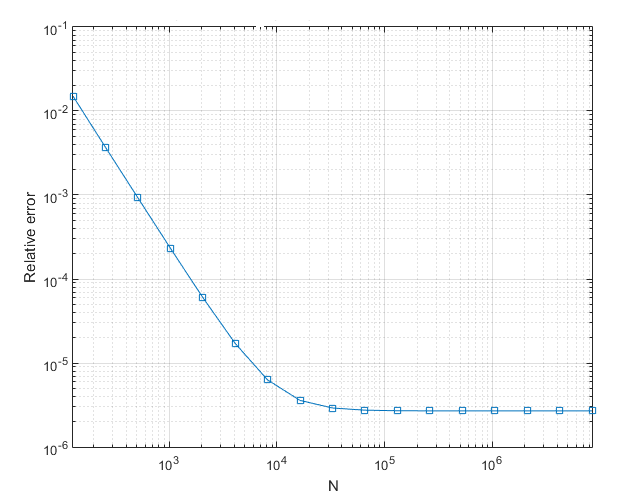
\includegraphics{2.png} 
\caption{Relative error of the method}
\end{figure}
\section{Second framework: integration by par parts }

The methods that were previously developed have shown to have good overall average approximation of the option price. However, another method looks to be interesting especially when the fourier transform of the payoff for some option's type is difficult to be analytically defined.\\
With the integration by parts approach, instead of caculating the fourier transform, we just need to  determine the integral of the payoff.~Very often, this integral brings more regularity to the approximation (barrier option , European option) , this regularity will improve the rate of convergence of the method.\\

\textbf{ integration by parts Theorem }
\begin{equation*}
\int f(x) g'(x) dx =  [f(x) g(x)] - \int g(x) f'(x)  dx 
\end{equation*}

For our case the option price is always given by :
\begin{gather*}
\pi(x, \tau)=e^{-r\tau} \int_{\mathbb{R}}g(y)p_{\tau}(y-x)dy 
\end{gather*}
for a fixed value of x, we set $p_{\tau}(y-x)=F(y) $\\
Thus, 
\begin{align*}
&\int_{\mathbb{R}}g(y)p_{\tau}(y-x)dy =\int_{\mathbb{R}}g(y)F(y)dy\\
&=[F(y) G(y)]_{\mathbb{R}} - \int_{\mathbb{R}} G(y) f(y)  dy\\
&=[p_{\tau}(y) G(y)]_{\mathbb{R}} - \int_{\mathbb{R}} G(y) p'_{\tau}(y)  dy
\end{align*}

Where G(y) is the antiderivative of $g(y)$, and $p'_{\tau}(y)$ is the derivative of F(y).
We will see that the probability density can be truncated at some point$y^*$ with a negligible effect.Thus the price will be approximated by :

\begin{gather}
\pi=-e^{-r\tau}\int_{0}^{y^*} G(y) p'_{\tau}(y)  dy \nonumber \\
\simeq -e^{-r\tau} \Delta y \sum_{k=0}^{N-1}G(y_k) p'_{\tau}(y_k)
\label{N-point}
\end{gather} 
In order to have a price approximation, we need to calculate the primitive of the payoff and the derivative of the probability density. we have already extracted a vector of the density using the FFT technique applied on the characteristic function \eqref{destrib} .To obtain samples of the derivative of the probability density we can use an important property of the Fourier transform illustrated by :
\begin{gather*}
f'(x)= i \omega \cdot \hat{f}(\omega)
\end{gather*}
Thus, 
\begin{gather}
p'_T(x_j)= i \omega_j \cdot   \frac{1}{2 \pi} e^{- iw_{min} x_j} \text{FFT}\big ( e^{-i \Delta\omega x_{min} } \varphi(\omega_k) \big) ~~for~ 0 \leqslant j < N
\end{gather}

The main advantage of the integration by parts is bringing more regularity to the function on which we desire apply the Trapezoidal rule and thus improving the convergence of the method. Moreover, we could work with the second and the third derivatives of the density function.
\begin{align*}
&\int_{0}^{y^*}g(y)p_{\tau}(y-x)dy = -
\int_{0}^{y^*} G(y) p'_{\tau}(y)  dy
=\int_{0}^{y^*} {\cal{G}}(y) p''_{\tau}(y)dy
=-\int_{0}^{y^*} {\mathbb{G}}(y) p'''_{\tau}(y)dy
\end{align*}   

Every time we calculate the primitive of the payoff we are moving from a function that has not a  first derivative to a function that has and that is more regular than its derivative. 

\section{Evaluation of the method }

The total error $\epsilon$ of the integration by parts method can be split into three components as the previous method. What distinguish the integration by parts is its quadrature error,the fact that we are applying the trapezoidal rule on more regular function makes it converge faster and by regularity we mean a continuous function that has a first derivative function.

Generally the truncation and the FFT errors are dominated by the quadrature error. Thus, we expect the overall error of this method TO converge faster than the previous one.

The first graph represents the relative error of the integration by parts computed with Anderson and Andersen parameters. Here we can remarkably see that the total error converges within $N = 10^3 < 10^4 $ and stabilize  approximately in $\epsilon=10^-7$\\

The second graph proves the effect of the gain in regularity.As we moved from a differentiable to a twice differentiable function, we can see that for the range of quadrature points such that $N > 10^3$ the integration by parts is faster than before

\begin{figure}[H]

\centering
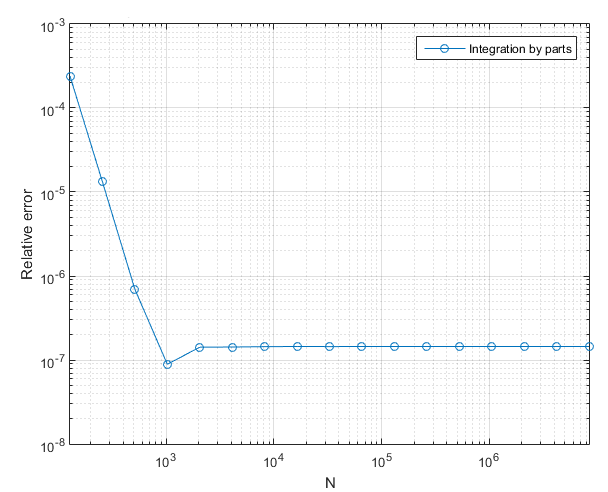
\includegraphics[scale=0.7]{Integrationbp.png} 
\caption{Error of the integration by parts method}
\end{figure}
 
\begin{figure}[H]

\centering
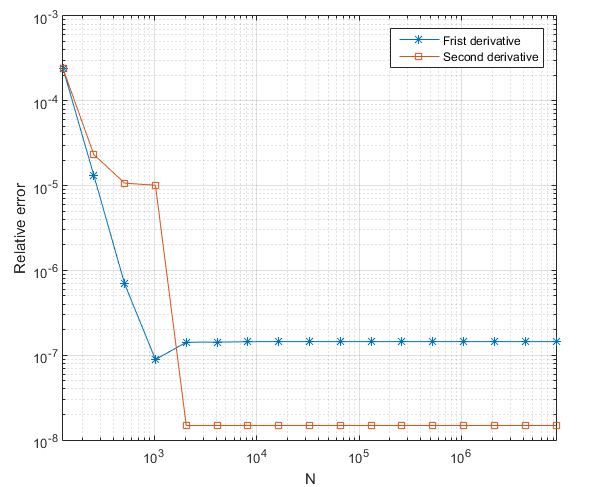
\includegraphics[scale=0.7]{1st2nd.png} 
\caption{Comparing the first and the second derivative}
\end{figure}
\chapter{Conclusion }
We have seen that a European option price can be obtained via samples of the characteristic function and the Fourier Transform of the payoff. Instead of computing an integral that involves the inner product of the terminal payoff and the density function we compute the integral of the inner product of the  Fourier transforms of these two components. This is convenient because in some cases the Levy process is known by its characteristic function.

[the characteristic function  of the Levy process is easier to be handled than the density function itself.]\\

\newpage
\appendix
\section{Appendix 4.5} \label{App:AppendixA}
In the following part we detail the expression of $f(x,\tau)$ used in chapter 4 equation \eqref{moneq}
\begin{align*}
f(x,\tau)=& e^{-r\tau}\expp{g \parent{X_T}|X_{T-\tau} = x}\\
&=\expp{g \parent{X_T}|X_{t} = x}\\
&=\int_{-\infty}^{\infty}g(y)p(X_T =y|X_t = x) dy 
\end{align*}
Here we develop the expression of the the conditional probability density based on Levy processes properties:
\begin{align*}
p(X_T =y|X_t = x,X_0=0)=&\frac{p(X_T-X_{T-\tau}=y-x)\cap p(X_{T-\tau}=x)}{ p(X_{T-\tau}=x)}\\
=&\frac{p(X_T-X_{T-\tau}=y-x) \cdot p(X_{T-\tau}=x)}{ p(X_{T-\tau}=x)},~ \text{Independent increments}\\
=&p(X_T-X_{T-\tau}=y-x),~ \text{Stationary increments}\\
=&p_{T-(T-\tau)}(y-x)\\
=&p_{\tau}(y-x)
\end{align*}
\section{Appendix } \label{App:AppendixB}
In the following part we detail the expression of $\hat{g}_{\alpha}$
\begin{align*}
\hat{g}_{\alpha}=&\int_{\mathbb{R}} e^{i\omega x}e^{-\alpha x}g(x)dx\\
=&\int_{\mathbb{R}} e^{(i\omega+\alpha) x}(S_0(e^x-e^k))\\
=& S_0 \int_{k}^{\infty} e^{(i\omega+\alpha) x}(e^{x}-e^{k})\\
=& S_0 \frac{e^{(1-\alpha+i\omega)k}}{(1+i\omega-\alpha)(i \omega-\alpha)}=& S_0 \int_{k}^{\infty} e^{(i\omega+\alpha) x}(e^{x}-e^{k})\\
=& S_0 \frac{e^{(1-\alpha+i\omega)k}}{(1+i\omega-\alpha)(i \omega-\alpha)}
\end{align*}

\newpage

 \begin{thebibliography}{1}
  \bibitem{notes} Hull.J.C. {\em options futures and other derivatives ($7^{th}$ edition)}  2009.
\bibitem{NOTES}Merton. R.C.{option Pricing when the underlying stock returns are discontinuous} 1976
\bibitem{notes}Cont.R and Tankov.P {\em Financial Modelling with Jump processes}
\bibitem {notes} Wang.W {\em Risk-neutral Approach to
Lévy Processes in Financial Modelling}
\bibitem{notes} Joshi.M.S.{\em Log-type models, Homogeneity OF Option prices and Convexity}
\bibitem{notes} Stenger.F .{\em Numerical Methods
Based on Sinc andAnalytic Functions}
\bibitem{notes} Merton.R.C.{Option Pricing when the Underlying Stock Returns Are Discontinuous} 1975.
\bibitem{notes}  Andersen, L. and Andreasen, J. {\em Jump Diffusion Processes: Volatility Smile Fitting
and Numerical Methods for Option Pricing},2000.
\bibitem{notes} Trefethen.L and Weidman.J.A.C.{\em The Exponentially  Convergent  of Trapezoidal  Rule}.2013
\end{thebibliography}{1}
 
\end{document}